\documentclass{standalone}
\usepackage{tikz}
\usepackage{xcolor}
\usepackage{helvet}
\renewcommand{\familydefault}{\sfdefault}

\definecolor{col1}{HTML}{ff6666}
\definecolor{col2}{HTML}{6691ff}
\definecolor{col3}{HTML}{fcff66}

\ifdefined\flam
\else\def\flam{0}
\fi
\ifdefined\health
\else\def\health{0}
\fi
\ifdefined\instab
\else\def\instab{0}
\fi
\ifdefined\spec
\else\def\spec{ }
\fi

\begin{document}
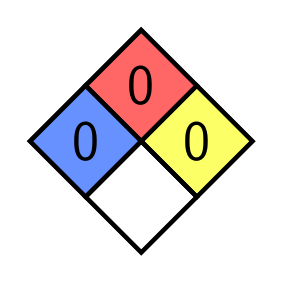
\begin{tikzpicture}[
		diamond/.style={ultra thick, rotate=45},
	]
	\huge
	\draw[diamond, fill=col1] (0,0) rectangle ++(1,1) node [midway, align=center] {\flam};
	\draw[diamond, fill=col2] (-1,0) rectangle ++(1,1) node [midway, align=center] {\health};
	\draw[diamond, fill=col3] (0,-1) rectangle ++(1,1) node [midway, align=center] {\instab};
	\Large
	\draw[diamond] (-1,-1) rectangle ++(1,1) node [midway, align=center] {\spec};
\end{tikzpicture}
\end{document}
